\subsection{Numerical Examples and Implications on Fairness}\label{sec:aggregation:imbalanced:numerical_examples}

\begin{figure}[tb]
	\centering
	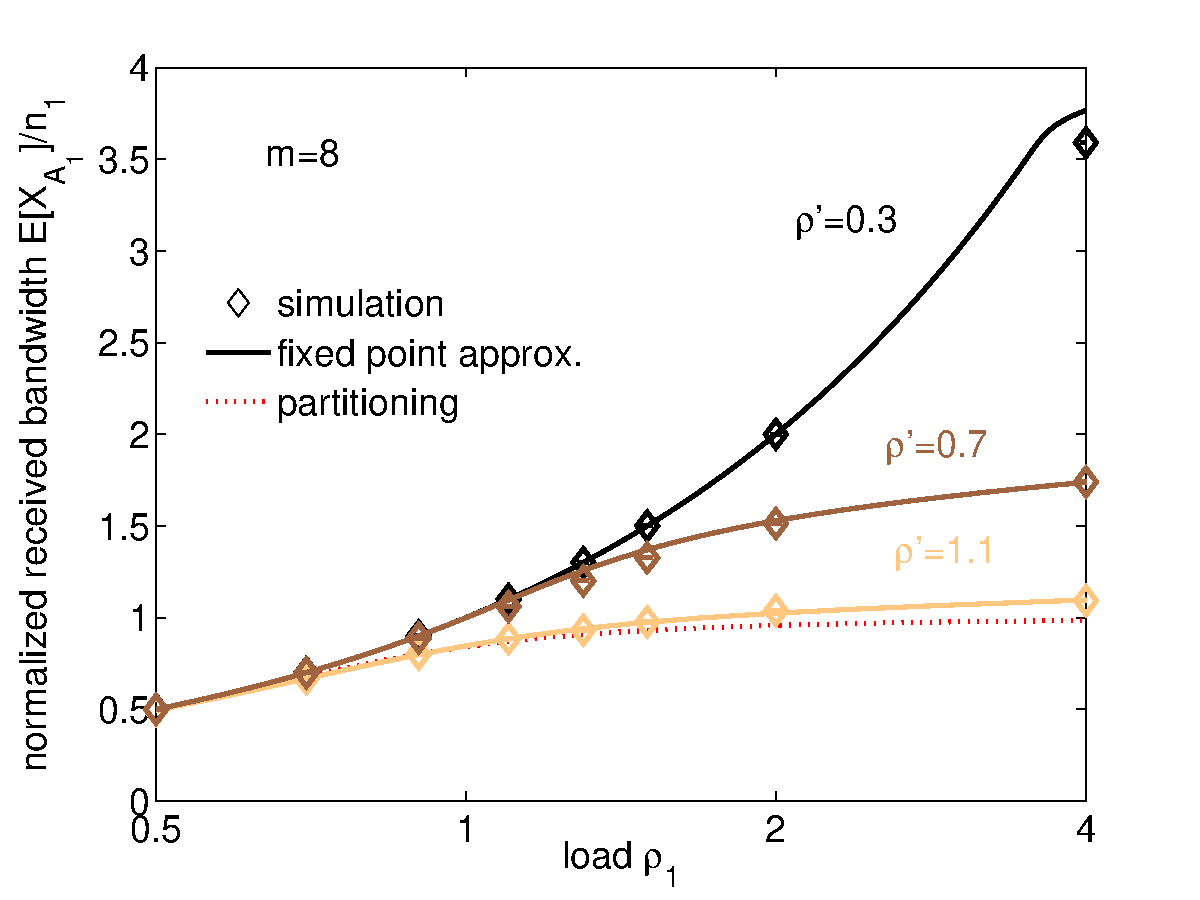
\includegraphics[width=0.7\textwidth]{aggregation/performance_model/figures/fp_bw_m8}
 	\caption{Received bandwidth $E[X_{A_1}]/n_1$ dependent on load of the other links $\rho'$ for $m=8$.}
 	\label{fig:bw_m8}
\end{figure}

\begin{figure}[tb]
	\centering
	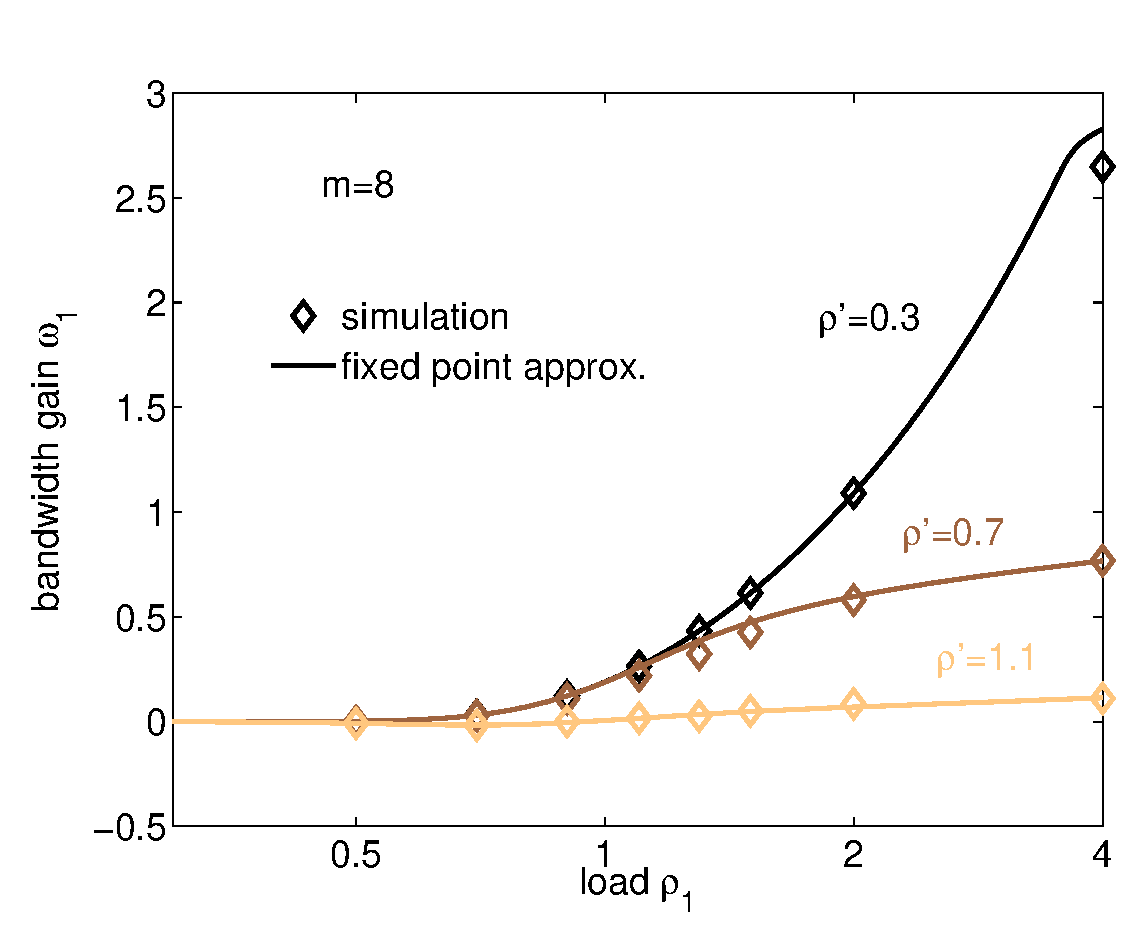
\includegraphics[width=0.7\textwidth]{aggregation/performance_model/figures/fp_bwgain_m8}
 	\caption{Bandwidth gain $\omega_1$ dependent on load of the other links $\rho'$ for $m=8$.}
 	\label{fig:bwgain_m8}
\end{figure}

The cooperating system can benefit if the load is heterogeneously distributed among the systems, such that a system which is currently busy can offload to an idle system.
%To investigate the performance in heterogeneous load conditions we calculate the blocking probability $p_{b_1}$ of the observed system dependent on its load $\rho_1$ and the load on the links in the composite system $\rho' = \rho_i, i\in\{2,\ldots,m\}$.

To assess the potential of bandwidth aggregation of $m$ systems in imbalanced load conditions, we study the load of the observed system $\rho_1$ and set the load of the other $m-1$ systems to the same value $\rho'$, i.e., $\rho_i=\rho',\forall i\in\{2,\dotsc,m\}$.
%As performance metric we consider the normalized received bandwidth of the observed system $E[X_{A_1}]/n_1$ and the bandwidth gain of the observed system $\omega_1$. We first investigate the impact of the impact of $\rho'$, then we investigate the number of cooperating systems $m$ for a fixed load $\rho'$.

\begin{figure}[tb]
	\centering
	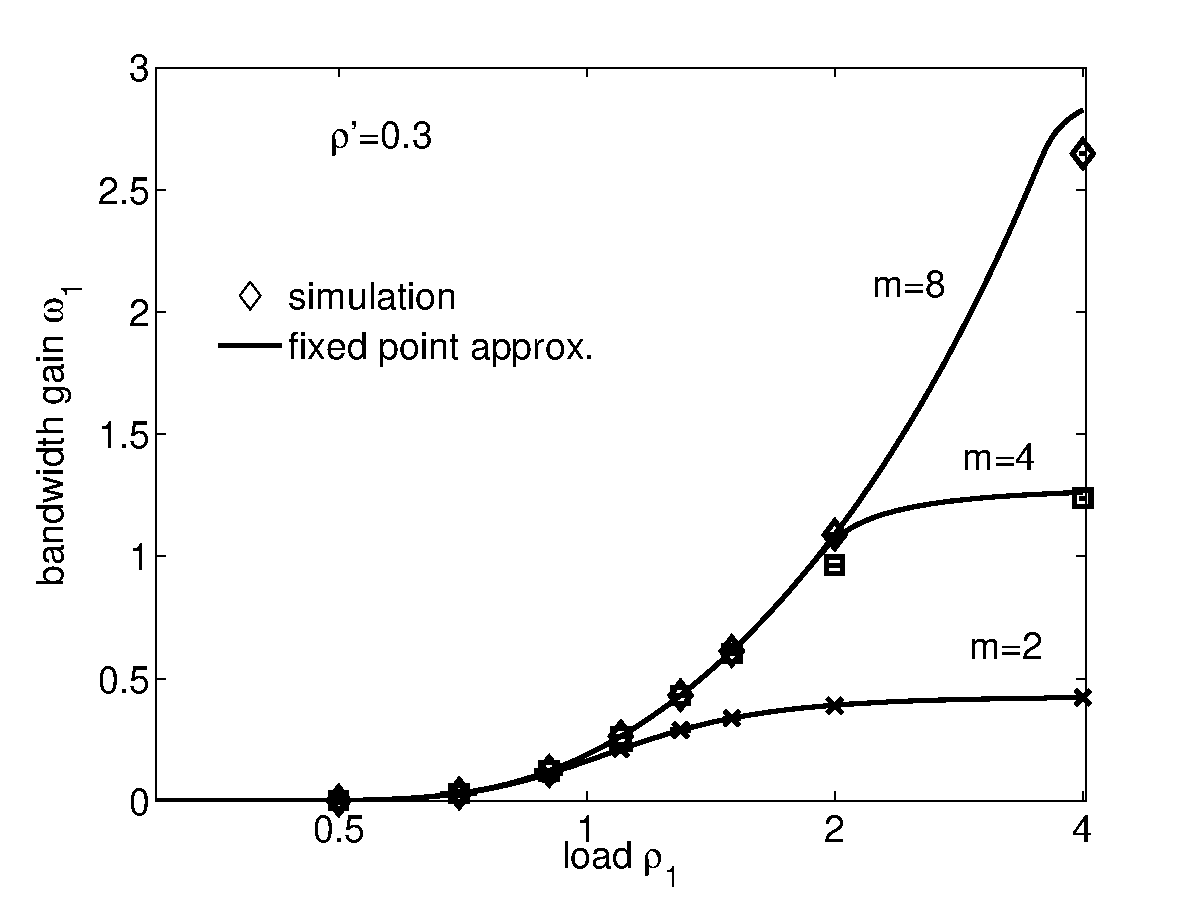
\includegraphics[width=0.7\textwidth]{aggregation/performance_model/figures/fp_bwgain_rho03}
 	\caption{Bandwidth gain dependent on load of the observed system in off peak operation ($\rho'=0.3$).}
 	\label{fig:fp_bwgain_rho03}
\end{figure}

\begin{figure}[tb]
	\centering
	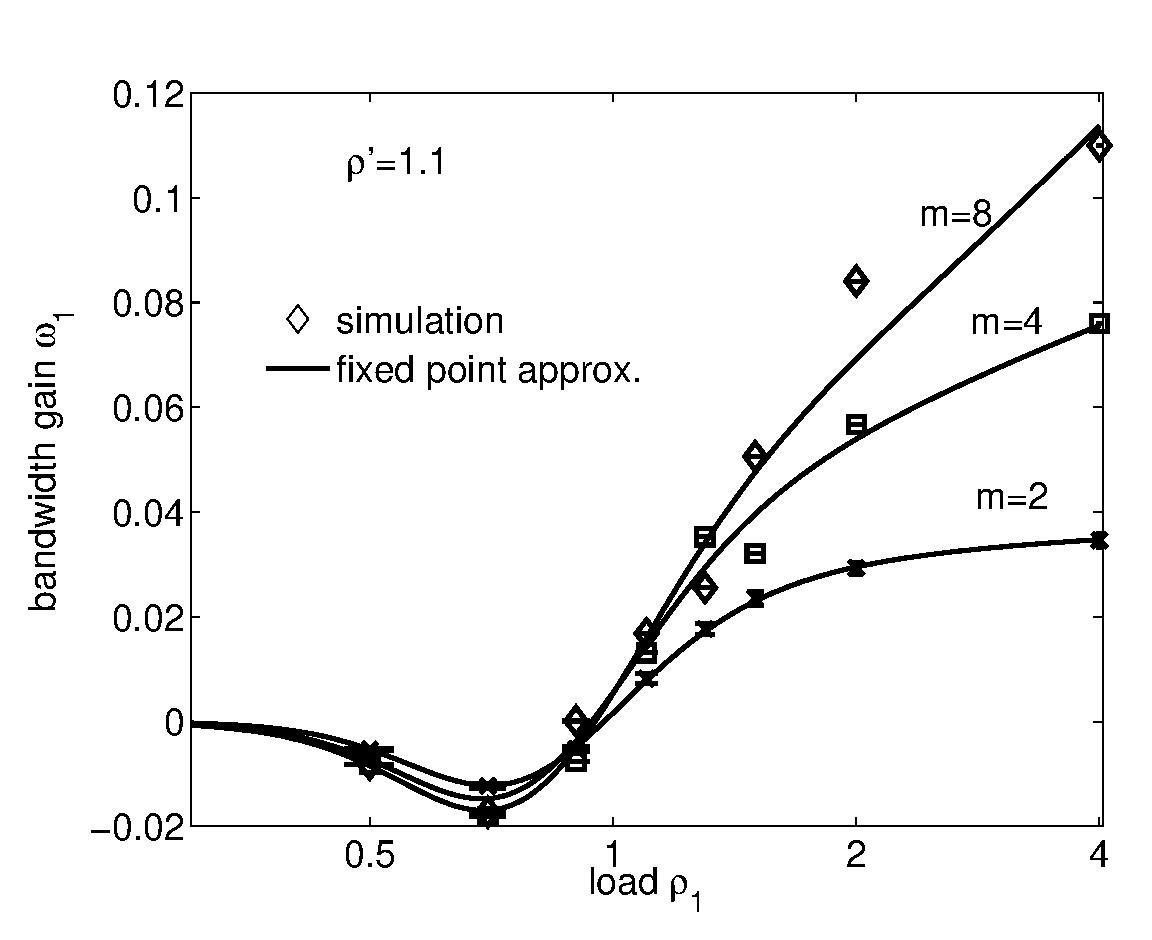
\includegraphics[width=0.7\textwidth]{aggregation/performance_model/figures/fp_bwgain_rho11}
 	\caption{Bandwidth gain dependent on load of the observed system in overload operation ($\rho'=1.1$).}
 	\label{fig:fp_bwgain_rho11}
\end{figure}

\begin{figure}[tb]
	\centering
	\includegraphics[width=0.7\textwidth]{aggregation/performance_model/figures/fp_bwgain_prio11}
 	\caption{Bandwidth gain dependent on load of the observed system in unfair operation ($\alpha_1 \neq \alpha'$).}
 	\label{fig:fp_bwgain_prio11}
\end{figure}

% \begin{figure*}[tb]
% \centering
% \begin{subfigure}{.49\textwidth}
%  \centering
%  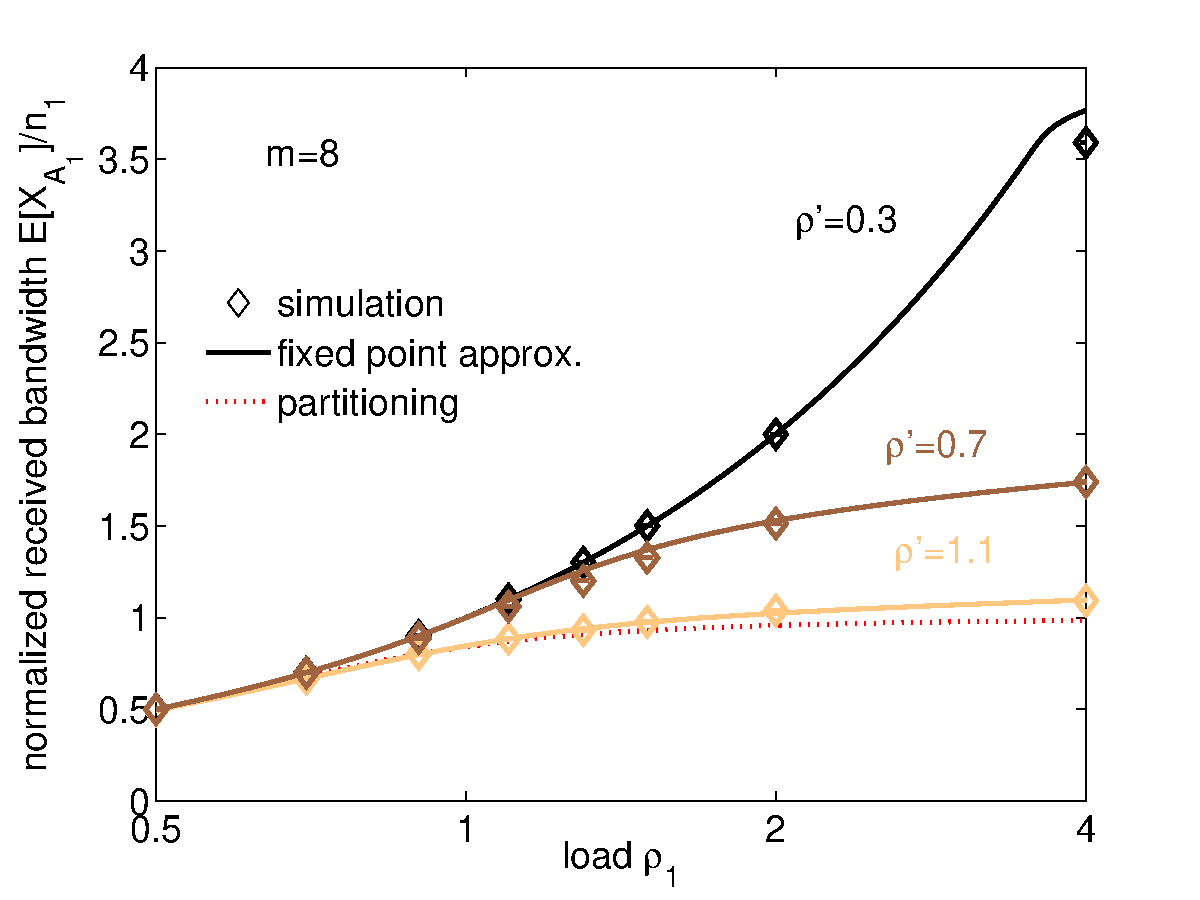
\includegraphics[width=\linewidth]{aggregation/performance_model/figures/fp_bw_m8}
%  \caption{Equal load}
%  \label{fig:bw_m8}
% \end{subfigure}%
% \begin{subfigure}{.49\textwidth}
%  \centering
%  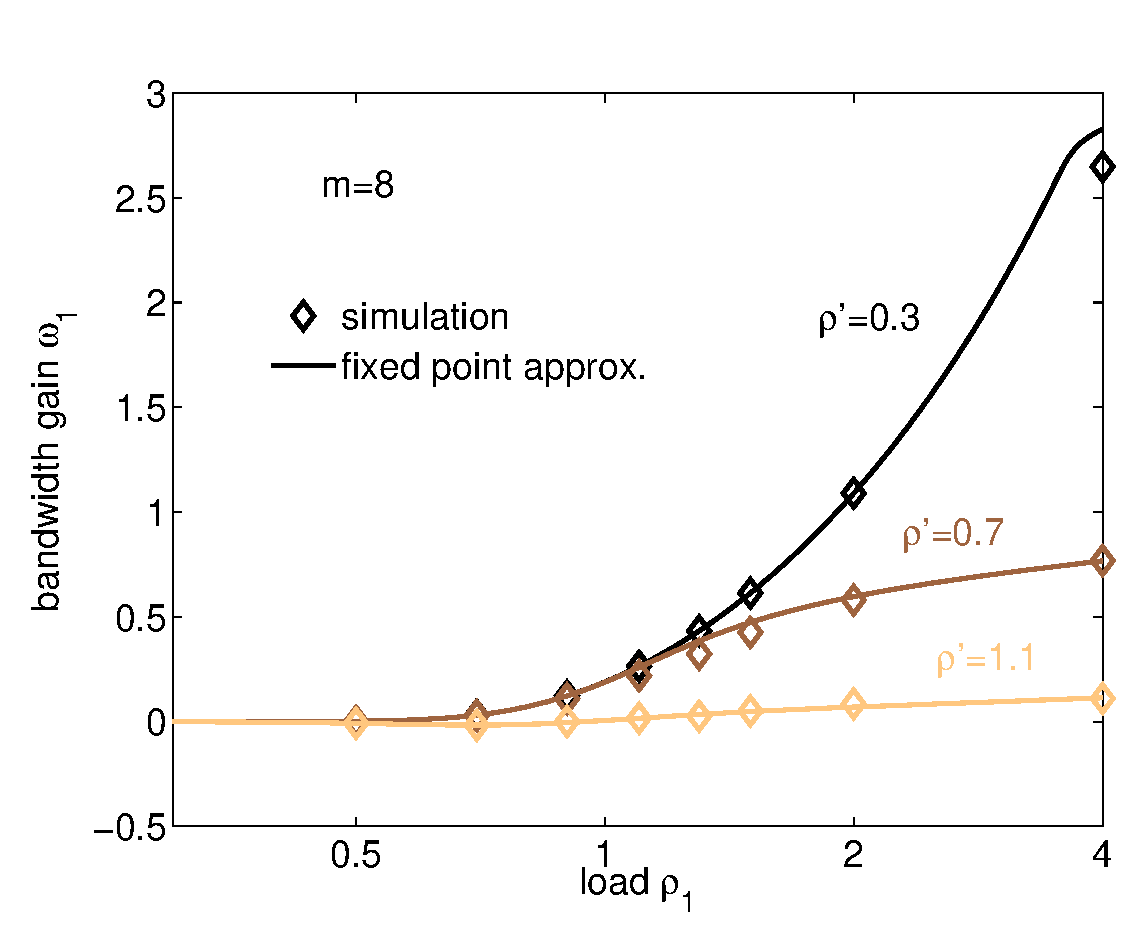
\includegraphics[width=\linewidth]{aggregation/performance_model/figures/fp_bwgain_m8}
%  \caption{bandwidth gain $\omega_1$}
%  \label{fig:bwgain_m8}
%  % 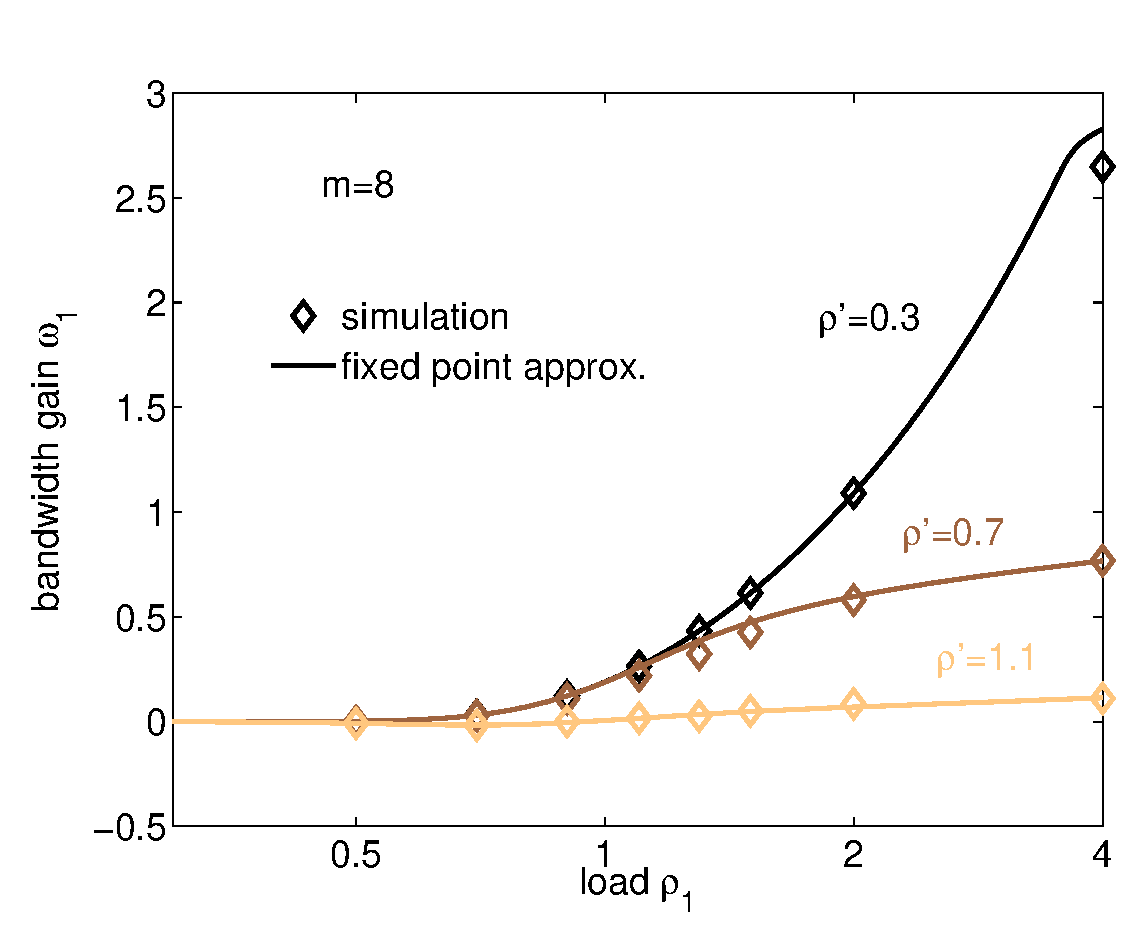
\includegraphics[width=\linewidth]{aggregation/performance_model/figures/fp_bwgain_m8}
%  % \caption{bandwidth gain $\omega_1$}
%  % \label{fig:bwgain_m8}
% \end{subfigure}
% \caption{Received bandwidth $E[X_{A_1}]/n_1$ dependent on load of the other links $\rho'$ for $m=8$}
% \label{fig:m8}
% \end{figure*}

In the following we investigate how the load on the links in the composite system $\rho'$ affects the throughput of the observed system for $m=8$ cooperating systems.
Figure~\ref{fig:bw_m8} shows the normalized received bandwidth of the observed system dependent on the throughput of the links in the composite system $\rho'$.
%The fixed point approximation decently fits the simulation results.
In case of $\rho'=0.3$ a lot of spare bandwidth is available for offloading. If the observed system is overloaded it can use the spare bandwidth and receives almost 400\% of its capacity if its offered load is 400\%. If the load $\rho'$ on the other links is higher, less bandwidth is available, which limits the received bandwidth. Still, the received bandwidth is above partitioning, although the links in the composite systems are overloaded with $\rho'=1.1$ if the observed system is even more overloaded.
%This can also be seen in the bandwidth gain $\omega_1$ depicted in Figure~\ref{fig:bwgain_m8}, which is positive if the observed system is overloaded with $\rho_1>1$. The bandwidth gain is only marginally negative, if the load on the observed system is low, which is manageable in off-peak periods. In busy periods the observed system benefits a lot by gaining more than 2.5 times more bandwidth if $\rho'=0.3$.

% \begin{figure*}[tb]
% \centering
% \begin{subfigure}{.7\textwidth}
%   \centering
%   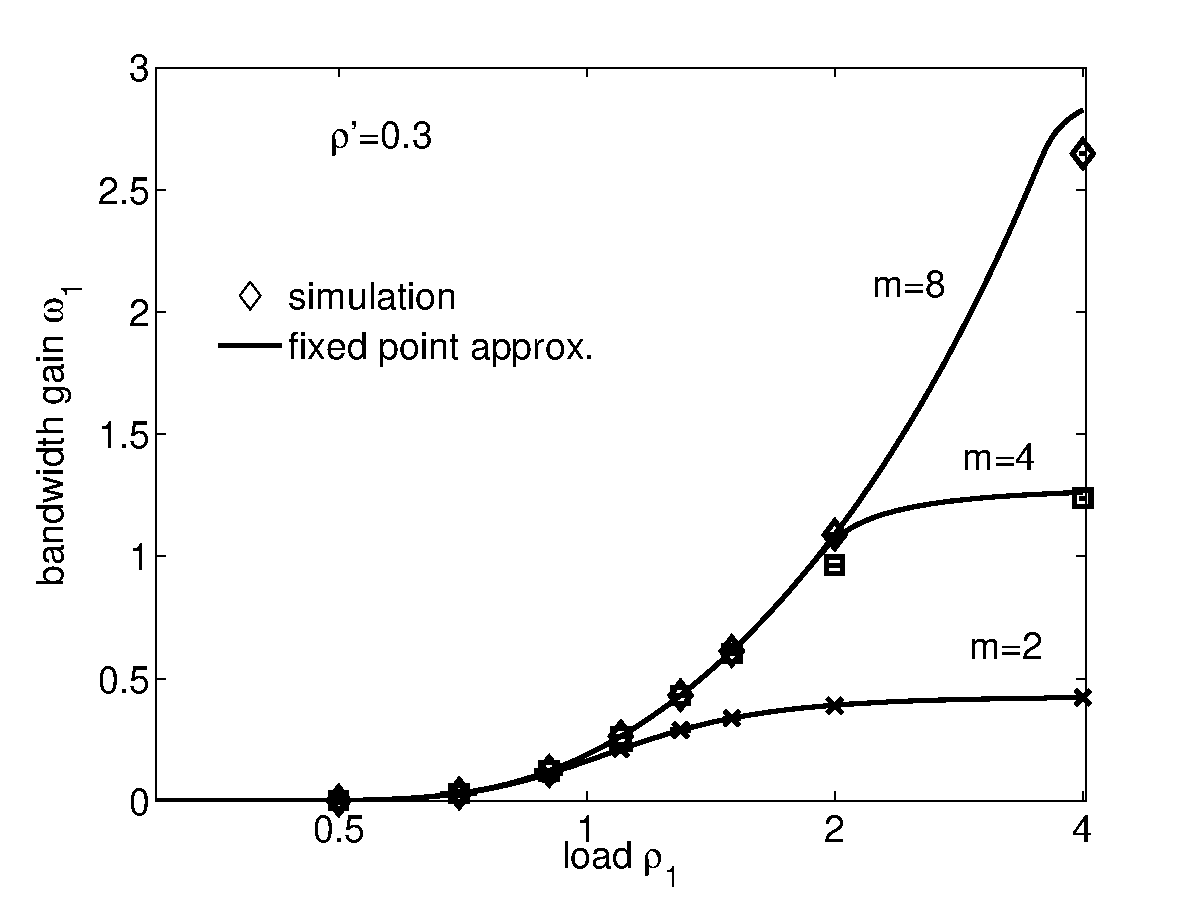
\includegraphics[width=\linewidth]{aggregation/performance_model/figures/fp_bwgain_rho03}
%   \caption{Off peak ($\rho'=0.3$)}
%   \label{fig:fp_bwgain_rho03}
% \end{subfigure}%
% \begin{subfigure}{.7\textwidth}
%   \centering
%   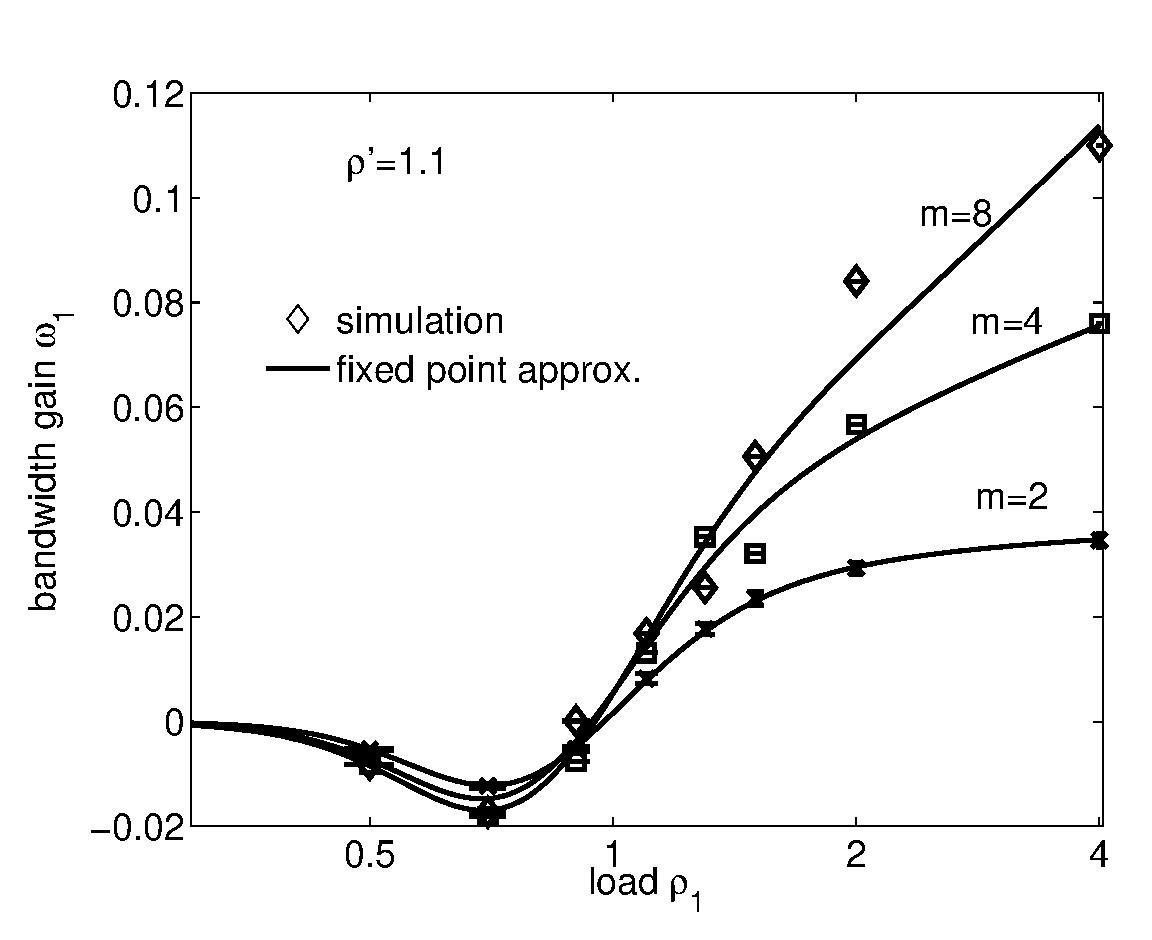
\includegraphics[width=\linewidth]{aggregation/performance_model/figures/fp_bwgain_rho11}
%   \caption{Overload ($\rho'=1.1$)}
%   \label{fig:fp_bwgain_rho11}
% \end{subfigure}
% \begin{subfigure}{.55\textwidth}
%   \centering
% \includegraphics[width=\linewidth]{aggregation/performance_model/figures/fp_bwgain_prio11}
%   	\caption{Unfair: ($\alpha_1 \neq \alpha'$)}
%   	\label{fig:fp_bwgain_prio11}
% \end{subfigure}
% \caption{Bandwidth gain dependent on load of the observed system in off peak, overload operation.} %and unfair operation.}
% \label{fig:fp_bwgain}
% \end{figure*}

\begin{figure}[tb]
	\centering
	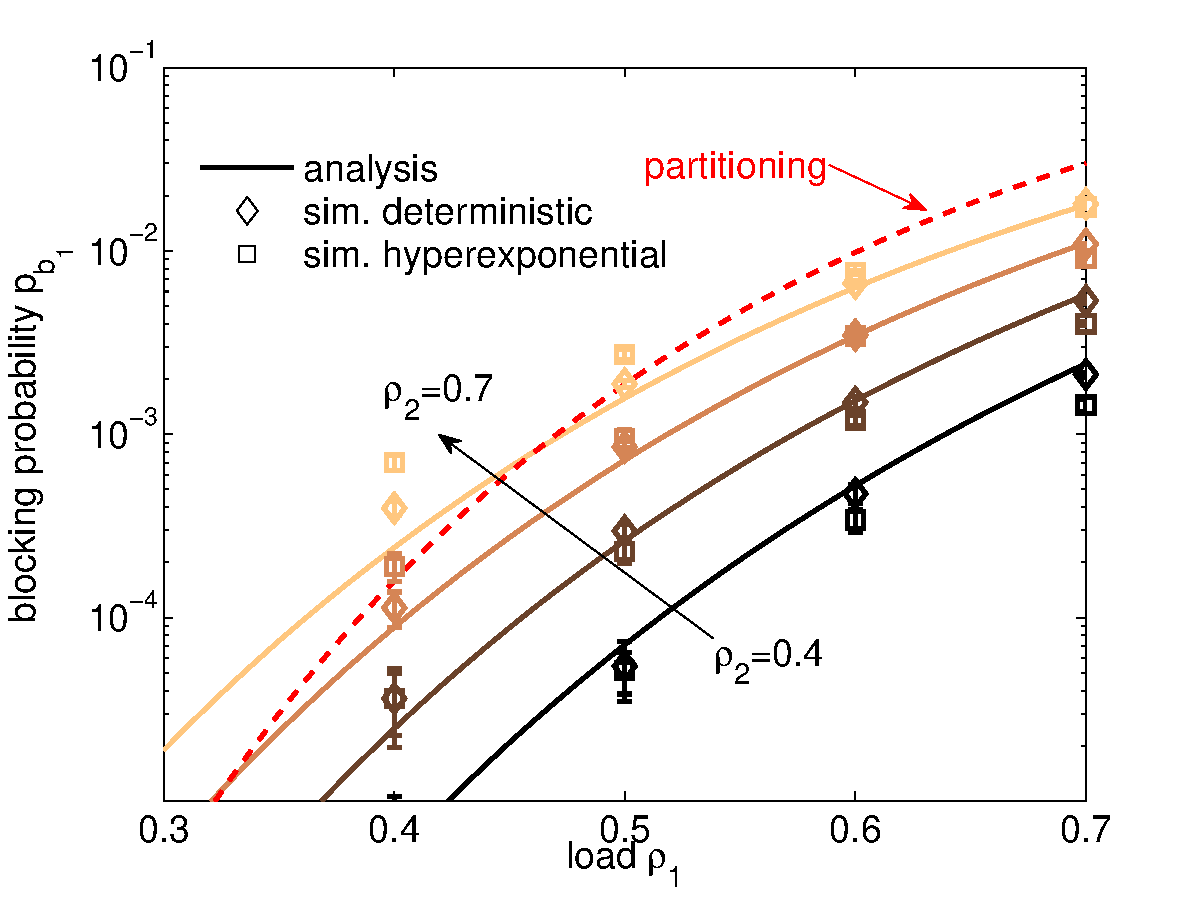
\includegraphics[width=0.7\textwidth]{aggregation/performance_model/figures/m2_n20_rho2_sim}
 	\caption{Blocking probability dependent on the load of reference and cooperating system. Simulation with different service time distributions.}
 	\label{fig:m2_n20_rho2_sim}
\end{figure}

\begin{figure}[tb]
	\centering
	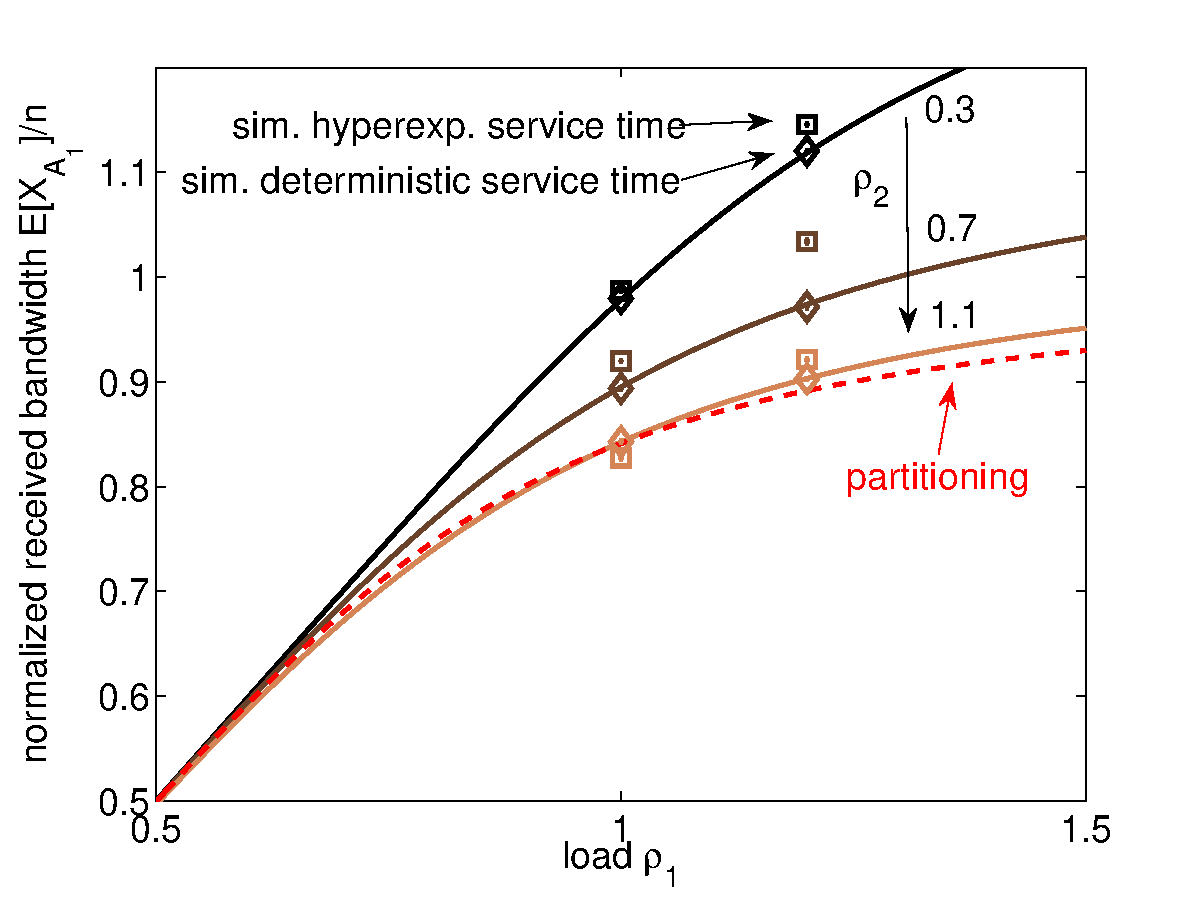
\includegraphics[width=0.7\textwidth]{aggregation/performance_model/figures/bw_n20_rho2_sim}
 	\caption{Received bandwidth dependent on the load of reference and cooperating system. Simulation with different service time distributions.}
 	\label{fig:bw_n20_rho2_sim}
\end{figure}

Figure~\ref{fig:fp_bwgain_rho03} shows the bandwidth gain of the observed system $\omega_1$ dependent on the number of cooperating systems $m$ for $\rho'=0.3$.
Hence, in this case there is a high potential to obtain spare bandwidth from the cooperating systems.
%Independent of the number of cooperating systems $m$, the bandwidth gain increases with the load $\rho_1$ on the observed system.
Depending on the number of cooperating systems the bandwidth gain of the observed system is limited.
%Up to a load of $\rho_1=1$, the spare bandwidth of one underutilized system with $\rho'=0.3$ is enough to support the observed system, which achieves the same bandwidth gain as with more cooperating systems.
%The bandwidth gain is equal for 4 and 8 cooperating systems up to a load of $\rho_1=2$.
%For higher loads of the observed system, the bandwidth that can be provided by 4 cooperating links reaches its limit.
%Especially if the number of cooperating systems is high, an overloaded system gains a lot of bandwidth.

Figure~\ref{fig:fp_bwgain_rho11} shows the bandwidth gain of the observed system $\omega_1$ dependent on the number of cooperating systems $m$ for $\rho'=1.1$.
In this case the links in the composite system are overloaded.
This leads to a loss of up to 2\% bandwidth if the observed system is not overloaded itself.
If the load on the observed system is high, but low enough that it supports other systems, a traffic burst is more likely to block the system, since the overall load on the systems is higher than in partitioning case.
%If the observed system is also overloaded its bandwidth gain increases dependent on the number of cooperating systems.

To conclude, if the load on the other systems is low, an overloaded system can highly profit from their spare bandwidth by gaining multiples of its own bandwidth. The maximum bandwidth gain is limited by the number of cooperating systems $m$.
If the cooperating systems are overloaded, the received bandwidth might be up to 2\% lower in some cases, but this is compensated with multiples of the base level bandwidth in high peak periods.

%\begin{figure}[tb]
%	\centering
% 	\includegraphics[width=0.5\textwidth]{figures/fp_bwgain_prio11}
%  	\caption{Bandwidth gain dependent on the load of the observed system in egoistic ($\alpha_1$=0\%,$\alpha'$=70\%), normal ($\alpha_1$=70\%,$\alpha'$=70\%) and altruistic ($\alpha_1$=70\%,$\alpha'$=0\%) operation.}
%  	\label{fig:fp_bwgain_prio11}
%\end{figure}

To prevent a system from being congested from an overloaded cooperating system, it can be prioritized. One possibility of prioritizing is to decrease the support threshold $\alpha$, so that it still can offload to other systems, but shares less bandwidth fractions to support. Figure~\ref{fig:fp_bwgain_prio11} shows the bandwidth gain of the observed system for three cases. The dotted line shows the blocking probability if observed and other systems have equal support threshold $\alpha_1=\alpha'=70\%$. The solid line shows the case where the observed system is altruistic and keeps its threshold at $\alpha_1=70\%$, but interacts with egoistic cooperating systems with support threshold $\alpha'=0\%$. The dashed line shows the egoistic case where the observed system limits its support threshold to $\alpha_1=0\%$, while the cooperating systems support up to $\alpha'=70\%$. The altruistic system suffers from egoistic cooperating systems by losing up to about 3\% bandwidth while not being able to gain bandwidth in high loads. Compared to that, the bandwidth gain in the egoistic case is never negative.
Hence, if a system is egoistic it always gains more bandwidth. However, the gain compared to normal operation is not high, and if each system would be egoistic no bandwidth can be shared. This would mean completely partitioned systems which would not change the current situation without bandwidth sharing.
On the other hand, if a system is the only one sharing among only free riders, which corresponds to the altruistic case, the situation is not worse, since only about 3\% of the bandwidth are lost.
Thus it is a win-win situation if everybody contributes to the system and shares spare bandwidth.
This provides incentives for systems to contribute.
%However, losing only up to about 3\% bandwidth in the case, where $m-1=7$ egoistic systems with high load ($\rho'=1.1$) are trying to exploit an altruistic system, shows that the mechanism is quite robust against free riders.
%The gain of the egoistic system decreases with the load of the cooperating system.
%Hence, prioritizing is only viable if the cooperating system is highly loaded.

\subsection{Simulation with Generally Distributed Service Times}\label{sec:simgeneral}

To assess the system performance in more general cases we run simulations with different service time distributions.
Figure~\ref{fig:m2_n20_rho2_sim} shows the blocking probability of the reference system dependent on the load of the systems. The mean values with 95\% confidence intervals of 8 simulation runs are plotted for the service time distributions deterministic and hyper-exponential.
The service times in the deterministic process are constant.
In the hyper-exponential process we use two branches with probabilities 10\% and 90\%.
For constant service times the blocking probability does not differ from the analytic model for high system loads. The blocking probability differs slightly from the analytic model for deterministic service times in low system loads, showing higher blocking probabilities if the load on the cooperating system is high. The reason for this has to be investigated and is part of future work. In case of the hyper-exponential distribution the service times are highly variant. Here the system which is highly loaded benefits from lower blocking probabilities compared to the analytic model.

% \begin{figure*}[tb]
% \centering
% \begin{subfigure}{.49\textwidth}
%  \centering
%  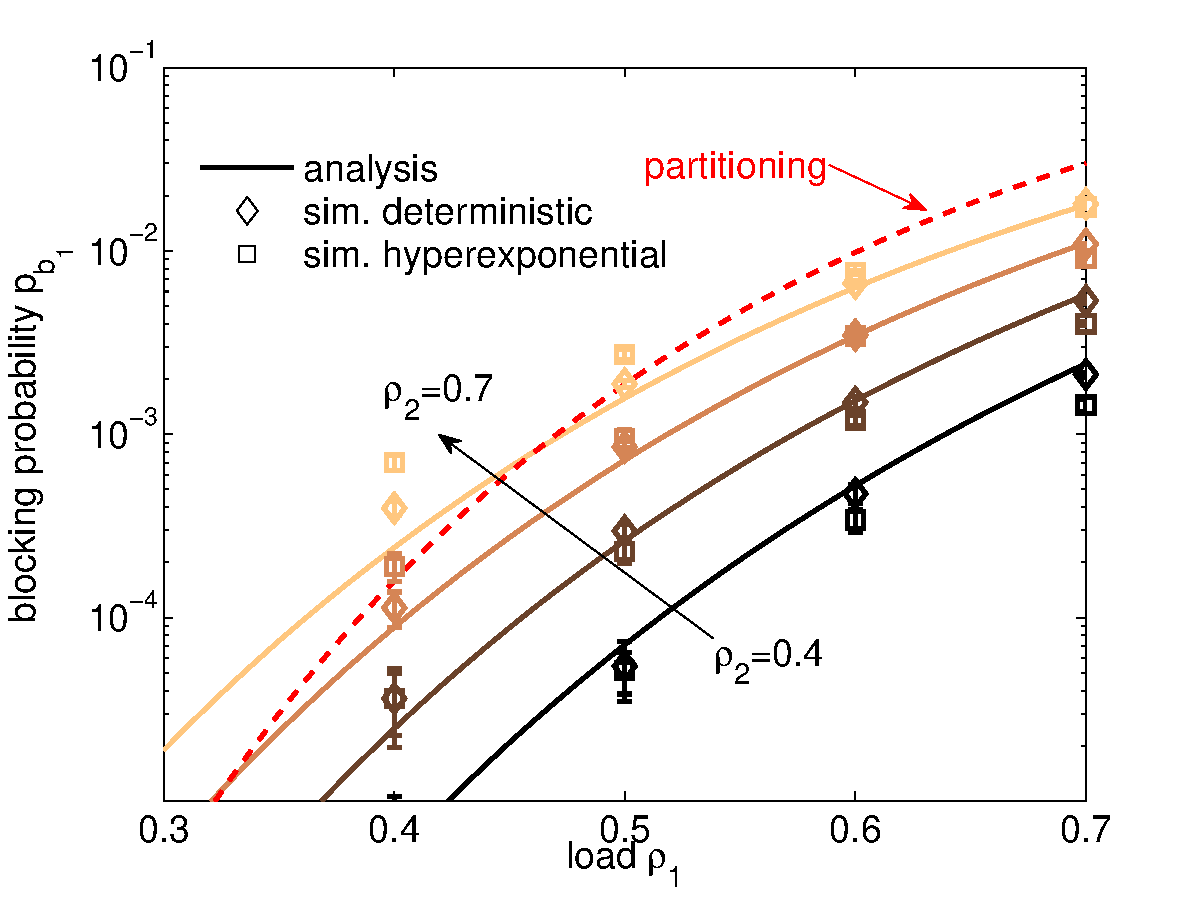
\includegraphics[width=\linewidth]{aggregation/performance_model/figures/m2_n20_rho2_sim}
%  \caption{Blocking probability}
%  \label{fig:m2_n20_rho2_sim}
% \end{subfigure}%
% \begin{subfigure}{.49\textwidth}
%  \centering
%  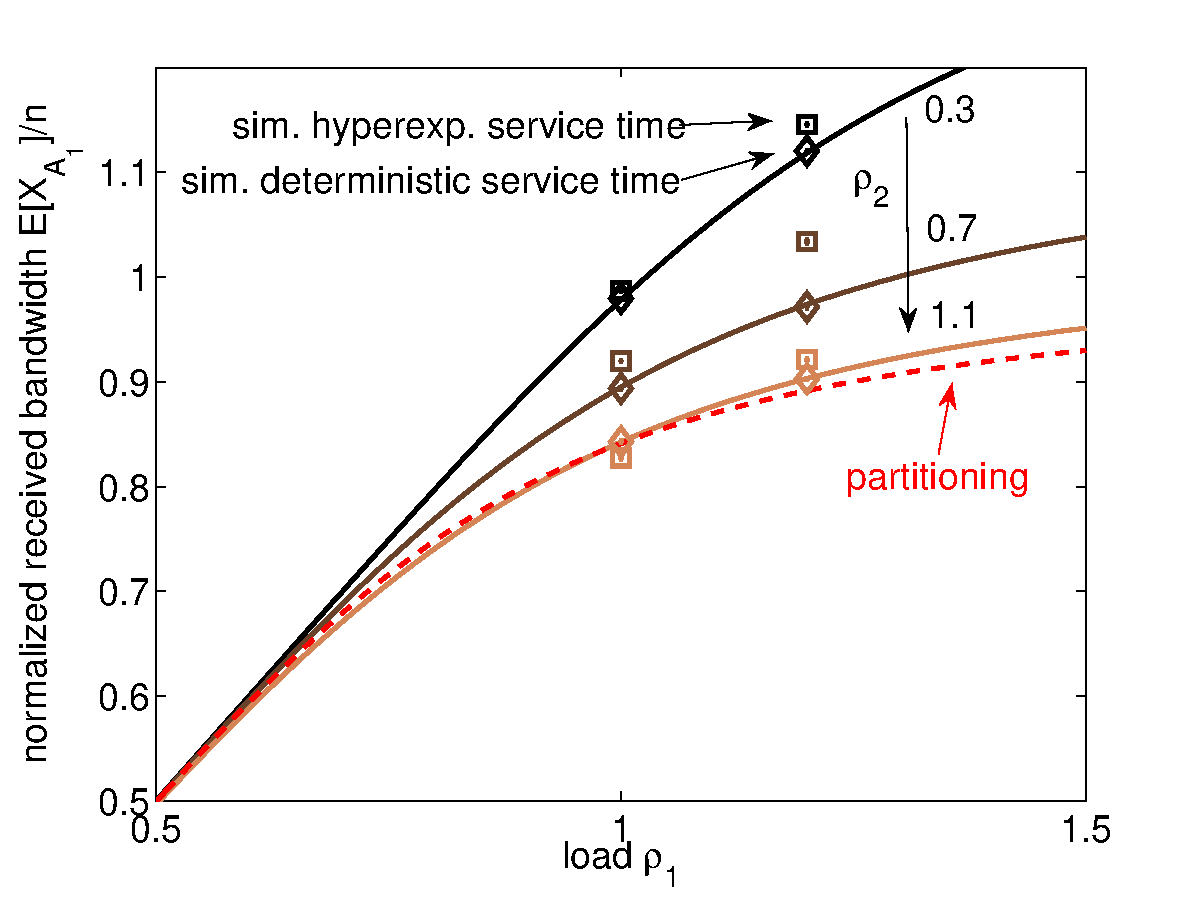
\includegraphics[width=\linewidth]{aggregation/performance_model/figures/bw_n20_rho2_sim}
%  \caption{Received bandwidth}
%  \label{fig:bw_n20_rho2_sim}
% \end{subfigure}
% \caption{Blocking probability and received bandwidth dependent on the load of reference and cooperating system. Simulation with different service time distributions.}
% \label{fig:n20_rho2_sim}
% \end{figure*}

In Figure~\ref{fig:bw_n20_rho2_sim}, which shows the received bandwidth of the reference system dependent on the load, simulation results are plotted for deterministic distributed and highly variant hyper-exponential distributed service times.
For deterministic service times the analytic model fits the simulation results. If the service times are highly variant the reference system receives only slightly more bandwidth than in the model if it is overloaded. Hence, considering the available bandwidth the analytic model can be used to assess the system performance with general service time distributions.

% \begin{figure}[tb]
% 	\centering
% 	\includegraphics[width=0.5\textwidth]{aggregation/performance_model/figures/m2_n20_q1}
%  	\caption{Blocking probability of two queues dependent on load.}
%  	\label{fig:m2_rho2_q1}
% \end{figure}
